\section{Criar CDevs} %%%%%%%%%%%%%%%%%%%%%%%%%%%%%%%%%%%%%%%%%%%%%%%%%%%%%%%

\subsection*{Introdução} %%%-----------------------------------------


\begin{frame}
	\frametitle{\textit{Character devices}}
	\begin{itemize}
		\item<1-> Vamos criar um driver de dispositivo de caractere.
		\item<2-> Esse dispositivo (scull) irá atuar sobre uma área da memória.
		\item<3-> A ideia é demonstrar a interface entre o \textit{kernel} e o dispositivo.
	\end{itemize}
\end{frame}


\begin{frame}
	\frametitle{\textit{Design} do dispositivo}
	\begin{itemize}
		\item<1-> Primeiro, iremos definir as capacidades (o mecanismo) que dispositivo irá disponibilizar para os programas.
		\item<2-> Serão criados os seguintes tipos de dispositivos:
		\begin{itemize}
			\item<3-> \textbf{scull0} a \textbf{scull3}: Área global e persistente da memória, acessível aos programas.
			% \item<4-> \textbf{scullpipe0} a \textbf{scullpipe3}: Dispositivos FIFO, onde um processo lê o que outro grava.
			% \item<5-> \textbf{scullsingle}, \textbf{scullpriv}, \textbf{sculluid} e \textbf{scullwuid}: Parecidos com \textit{scull0}, porém regras para a abertura do dispositivo.
		\end{itemize}
	\end{itemize}
\end{frame}


\begin{frame}
	\frametitle{Números Maiores e Menores}
	\begin{itemize}
		\item<1-> Dispositivos de caractere são acessados pelo nome no sistema de arquivos.
		\item<2-> Eles são arquivos especiais localizados em \textit{/dev}.
		\item<3-> Dispositivos de caractere são identificados pela letra ``c'' (através do comando `\textit{ls -l}')
		\item<4-> Dispositivos de bloco são identificados pela letra ``b''
	\end{itemize}
\end{frame}


\begin{frame}[fragile]
	\frametitle{Números Maiores e Menores}
	\begin{itemize}
		\item<1-> Os dois números que aparecem antes da data de modificação são os números de identificação do dispositivo:
		\begin{itemize}
		
			\note[item]<1> {Esses são os significados tradicionais para esses números.}
			
			\item<1-> \textit{\textbf{Major Number}}: Identifica o driver associado ao dispositivo;
			\item<1-> \textit{\textbf{Minor Number}}: Usado pelo \textit{kernel} para identificar o dispositivo referenciado.
		\end{itemize}
	\end{itemize}
		
	\lstset{language=TeX, numbers=none}
	\begin{block}<1->{}
	\begin{lstlisting}
	    crw-rw-rw- 1 root root  1,   3 Apr 11 2002  null
	    crw------- 1 root root 10,   1 Apr 11 2002  psaux
	    crw------- 1 root root  4,   1 Oct 28 03:04 tty1
	    crw-rw-rw- 1 root tty   4,  64 Apr 11 2002  ttys0
	    crw-rw---- 1 root uucp  4,  65 Apr 11 2002  ttyS1
	    crw--w---- 1 vcsa tty   7,   1 Apr 11 2002  vcs1
	    crw--w---- 1 vcsa tty   7, 129 Apr 11 2002  vcsa1
	    crw-rw-rw- 1 root root  1,   5 Apr 11 2002  zero
	\end{lstlisting}
	\end{block}
	
\end{frame}


\subsection*{Estruturas} %%%-----------------------------------------


\begin{frame}[fragile]
	\frametitle{\textit{Character devices}}
	
	\begin{itemize}
		\item<1-> Para criar um driver de dispositivo de caractere precisamos codificar alguns métodos e ligá-los através das estruturas (ver \cite{LinuxDrivers} e \cite{LDD3_3x}):
		\begin{itemize}
			\item<1-> file\_operations
			\item<1-> seq\_operations
		\end{itemize}
	\end{itemize}

	\lstset{language=C}
	
	\begin{block}<1->{}
		\begin{lstlisting}
			static struct file_operations scull_proc_ops = {
			  .owner   = THIS_MODULE,
			  .open    = scull_proc_open,
			  .read    = seq_read,
			  .llseek  = seq_lseek,
			  .release = seq_release
			};
		\end{lstlisting}
	\end{block}

\end{frame}


\begin{frame}[fragile]
	\frametitle{\textit{Character devices}}
	
	\lstset{language=C}

	\begin{block}<1->{}
		\begin{lstlisting}
			struct file_operations scull_fops = {
			  .owner   = THIS_MODULE,
			  .llseek  = scull_llseek,
			  .read    = scull_read,
			  .write   = scull_write,
			  .unlocked_ioctl = scull_ioctl,
			  .open    = scull_open,
			  .release = scull_release,
			};
		\end{lstlisting}
	\end{block}

	\begin{block}<1->{}
		\begin{lstlisting}
			static struct seq_operations scull_seq_ops = {
			  .start = scull_seq_start,
			  .next  = scull_seq_next,
			  .stop  = scull_seq_stop,
			  .show  = scull_seq_show
			};
		\end{lstlisting}
	\end{block}

\end{frame}


\begin{frame}
	\frametitle{\textit{Scull Device}}
	\begin{itemize}
		\item<1-> Estrutura do dispositivo criado:
	\end{itemize}
	\begin{columns}[T]
		\begin{column}{.15\textwidth}
		\end{column}
		\begin{column}{.7\textwidth}
			\uncover<1-> {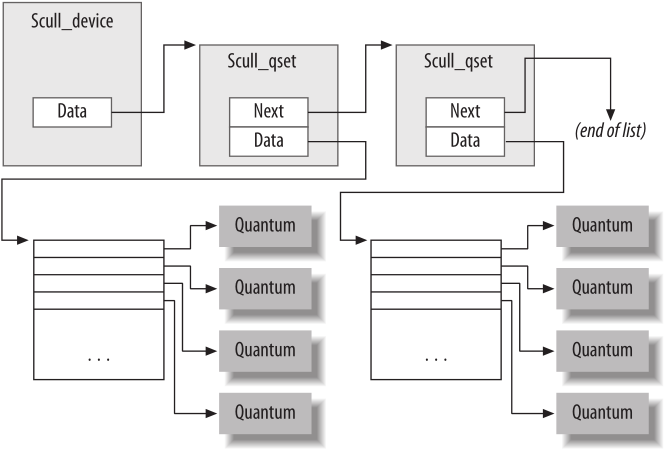
\includegraphics[width=\textwidth]{LayoutScull} \tiny{\cite{LinuxDrivers}}}
		\end{column}
		\begin{column}{.15\textwidth}
		\end{column}
	\end{columns}
\end{frame}


\begin{frame}[fragile]
	\frametitle{\textit{Método de criptografia XOR}}
	
	\begin{itemize}
		\item<1-> Exemplo de criptografia dos caracteres (inserido no método Write) \cite{Codecall_XOR}:
	\end{itemize}
	
	\lstset{language=C}

	\begin{block}<1->{}
		\begin{lstlisting}
			ssize_t scull_read(struct file *filp, char __user *buf, size_t count, loff_t *f_pos) {
			  // (...) Criptografa cada uma das letras da memoria
			  char key[21]   = "12345678901234567890";
			  int  key_count = 0; int  i; int  letra; int  chave;
			  char *buf_ok   = dptr->data[s_pos]+q_pos;
			  for (i=0 ; i<count ; i++)
			  {
			    letra  = buf_ok[i];
			    chave  = key[key_count];
			    buf_ok[i] = letra ^ chave;
			    key_count++;
			    if(key_count == strlen(key))
			      key_count = 0;
			  } // (...)
			}
		\end{lstlisting}
	\end{block}

\end{frame}
